%Version 3.1 December 2024
% See section 11 of the User Manual for version history
%
%%%%%%%%%%%%%%%%%%%%%%%%%%%%%%%%%%%%%%%%%%%%%%%%%%%%%%%%%%%%%%%%%%%%%%
%%                                                                 %%
%% Please do not use \input{...} to include other tex files.       %%
%% Submit your LaTeX manuscript as one .tex document.              %%
%%                                                                 %%
%% All additional figures and files should be attached             %%
%% separately and not embedded in the \TeX\ document itself.       %%
%%                                                                 %%
%%%%%%%%%%%%%%%%%%%%%%%%%%%%%%%%%%%%%%%%%%%%%%%%%%%%%%%%%%%%%%%%%%%%%

%%\documentclass[referee,sn-basic]{sn-jnl}% referee option is meant for double line spacing

%%=======================================================%%
%% to print line numbers in the margin use lineno option %%
%%=======================================================%%

%%\documentclass[lineno,pdflatex,sn-basic]{sn-jnl}% Basic Springer Nature Reference Style/Chemistry Reference Style

%%=========================================================================================%%
%% the documentclass is set to pdflatex as default. You can delete it if not appropriate.  %%
%%=========================================================================================%%

%%\documentclass[sn-basic]{sn-jnl}% Basic Springer Nature Reference Style/Chemistry Reference Style

%%Note: the following reference styles support Namedate and Numbered referencing. By default the style follows the most common style. To switch between the options you can add or remove “Numbered” in the optional parenthesis. 
%%The option is available for: sn-basic.bst, sn-chicago.bst%  
 
%%\documentclass[pdflatex,sn-nature]{sn-jnl}% Style for submissions to Nature Portfolio journals
%%\documentclass[pdflatex,sn-basic]{sn-jnl}% Basic Springer Nature Reference Style/Chemistry Reference Style
\documentclass[pdflatex,sn-mathphys-num]{sn-jnl}% Math and Physical Sciences Numbered Reference Style
%%\documentclass[pdflatex,sn-mathphys-ay]{sn-jnl}% Math and Physical Sciences Author Year Reference Style
%%\documentclass[pdflatex,sn-aps]{sn-jnl}% American Physical Society (APS) Reference Style
%%\documentclass[pdflatex,sn-vancouver-num]{sn-jnl}% Vancouver Numbered Reference Style
%%\documentclass[pdflatex,sn-vancouver-ay]{sn-jnl}% Vancouver Author Year Reference Style
%%\documentclass[pdflatex,sn-apa]{sn-jnl}% APA Reference Style
%%\documentclass[pdflatex,sn-chicago]{sn-jnl}% Chicago-based Humanities Reference Style

%%%% Standard Packages
%%<additional latex packages if required can be included here>

\usepackage{graphicx}%
\usepackage{multirow}%
\usepackage{amsmath,amssymb,amsfonts}%
\usepackage{amsthm}%
\usepackage{mathrsfs}%
\usepackage[title]{appendix}%
\usepackage{xcolor}%
\usepackage{textcomp}%
\usepackage{manyfoot}%
\usepackage{booktabs}%
\usepackage{algorithm}%
\usepackage{algorithmicx}%
\usepackage{algpseudocode}%
\usepackage{listings}%
\usepackage{tikz}%
\usetikzlibrary{shapes.geometric,arrows.meta,positioning,fit,backgrounds,calc}%
\usepackage{subcaption}%
\usepackage{float}%
%%%%

%%%%%=============================================================================%%%%
%%%%  Remarks: This template is provided to aid authors with the preparation
%%%%  of original research articles intended for submission to journals published 
%%%%  by Springer Nature. The guidance has been prepared in partnership with 
%%%%  production teams to conform to Springer Nature technical requirements. 
%%%%  Editorial and presentation requirements differ among journal portfolios and 
%%%%  research disciplines. You may find sections in this template are irrelevant 
%%%%  to your work and are empowered to omit any such section if allowed by the 
%%%%  journal you intend to submit to. The submission guidelines and policies 
%%%%  of the journal take precedence. A detailed User Manual is available in the 
%%%%  template package for technical guidance.
%%%%%=============================================================================%%%%

%% as per the requirement new theorem styles can be included as shown below
\theoremstyle{thmstyleone}%
\newtheorem{theorem}{Theorem}%  meant for continuous numbers
%%\newtheorem{theorem}{Theorem}[section]% meant for sectionwise numbers
%% optional argument [theorem] produces theorem numbering sequence instead of independent numbers for Proposition
\newtheorem{proposition}[theorem]{Proposition}% 
%%\newtheorem{proposition}{Proposition}% to get separate numbers for theorem and proposition etc.

\theoremstyle{thmstyletwo}%
\newtheorem{example}{Example}%
\newtheorem{remark}{Remark}%

\theoremstyle{thmstylethree}%
\newtheorem{definition}{Definition}%

\raggedbottom
%%\unnumbered% uncomment this for unnumbered level heads

\begin{document}

\title[Article Title]{A Communication-Realistic Sim-to-Sim Validation Framework for Reinforcement Learning Humanoid Locomotion Using Digital Twins}

\author*[1]{\fnm{Juan Andres} \sur{Mendez}}\email{ja.mendez@uniandes.edu.co}

\author[1]{\fnm{Carlos} \sur{Lozano-Garzon}}\email{calozanog@uniandes.edu.co}
\equalcont{These authors contributed equally to this work.}

\affil*[1]{\orgdiv{Systems and Computing Engineering Department}, \orgname{Universidad de los Andes}, \orgaddress{\street{Street}, \city{Bogota}, \postcode{100190}, \country{Colombia}}}


\abstract{Humanoid robot locomotion remains a challenging problem for reinforcement learning due to the complexity of high-degree-of-freedom articulated systems, safety risks during experimental training, and the persistent simulation-to-reality transfer gap. These challenges are particularly relevant in research and educational contexts where access to physical humanoid platforms is limited. This paper presents an integrated framework for developing and validating humanoid locomotion policies that combines digital twins, reinforcement learning training, and communication-realistic validation prior to hardware deployment. The proposed pipeline trains goal-directed locomotion policies for the Unitree G1 humanoid robot in a high-fidelity simulation environment using Proximal Policy Optimization operating on proprioceptive observations across 29 actuated degrees of freedom. To reduce deployment risks, the framework incorporates a simulation-to-simulation validation stage that evaluates trained policies using authentic ROS 2 middleware communication, enabling testing under realistic control conditions before execution on the physical robot. Experimental results demonstrate stable bipedal locomotion and achieve an 87\% goal success rate in point-to-point navigation tasks. Additional exploratory experiments on obstacle-aware navigation reveal important challenges in reward design when combining goal-seeking and collision-avoidance objectives. The proposed framework provides a practical methodology for safer and more reproducible reinforcement learning experimentation in humanoid robotics.}


\keywords{Humanoid Robots; Deep Reinforcement Learning; Robot Locomotion; simulation-to-reality transfer; Digital Twins; ROS 2 Middleware; Social Navigation}

%%\pacs[JEL Classification]{D8, H51}

%%\pacs[MSC Classification]{35A01, 65L10, 65L12, 65L20, 65L70}

\maketitle

\section{Introduction}
\label{intro}

Humanoid robots are among the most complex and promising domains in modern robotics. Their ability to operate in environments designed for humans makes them particularly attractive for applications ranging from service robotics to human–robot interaction and collaborative automation. However, achieving robust locomotion on humanoid platforms remains challenging due to the large number of degrees of freedom, nonlinear dynamics, and the need to maintain dynamic balance while interacting with complex environments \cite{bib1}, \cite{bib2}.

Recent advances in physics-based simulation and deep reinforcement learning (RL) have significantly expanded the possibilities for developing locomotion control policies in simulated environments prior to physical deployment. High-fidelity simulation platforms enable the creation of digital twins that replicate the kinematic structure, dynamics, and sensing capabilities of real robotic systems with greater realism \cite{bib3}. In parallel, reinforcement learning algorithms have demonstrated promising results in synthesizing locomotion behaviors for robots with complex articulated structures, allowing control policies to emerge through interaction with simulated environments rather than explicit programming \cite{bib4}.

Despite these advances, transferring learned policies from simulation to real robotic systems remains a significant challenge. This problem, commonly referred to as the simulation-to-reality (sim-to-real) gap, arises from discrepancies between simulated and physical environments, including modeling inaccuracies, sensor noise, actuator limitations, and environmental variability. Even small differences between simulation and reality can cause learned policies to degrade or fail when deployed on physical hardware.

An additional challenge arises from the fact that most reinforcement learning locomotion studies evaluate trained policies directly within simulation environments that bypass the software architectures used in real robotic systems. In practice, humanoid robots rely on middleware frameworks that manage communication between sensors, control modules, and actuators. These middleware layers introduce communication delays, message serialization, and asynchronous processing effects that are typically not represented during reinforcement learning training or evaluation. As a result, policies that perform well in native simulation environments may exhibit unexpected behavior when integrated with the software stacks used for real robotic deployment.

Addressing this validation gap is particularly important in research and educational environments where access to humanoid hardware platforms is limited and experimental failures can result in costly damage or extended system downtime. Under these constraints, development pipelines that enable extensive experimentation and validation prior to hardware deployment are essential for accelerating research while preserving the integrity of robotic platforms.

This paper proposes an integrated framework for training and validating humanoid locomotion policies that combines digital twins, deep reinforcement learning, and communication-realistic validation. The framework is implemented using a high-fidelity digital twin of the Unitree G1 humanoid robot and trains goal-directed locomotion policies using Proximal Policy Optimization operating directly on joint-level control actions. To reduce deployment risks, the proposed pipeline incorporates a simulation-to-simulation validation stage in which trained policies interact with the robot model through authentic ROS 2 middleware communication, reproducing the control architecture used in real robotic systems.

The proposed approach is evaluated through a set of locomotion experiments in which the robot learns goal-directed point-to-point navigation using proprioceptive observations across 29 actuated degrees of freedom. The learned policy achieves stable bipedal locomotion with an 87\% success rate in reaching navigation targets. In addition, exploratory experiments investigate the integration of LiDAR-based perception for obstacle-aware navigation. These experiments reveal important challenges in reward design when combining goal-seeking and collision-avoidance objectives, highlighting the complexity of multi-objective learning for humanoid navigation.

The contributions of this work are threefold:
\begin{enumerate}
    \item \textbf{A communication-realistic simulation-to-simulation validation framework} that evaluates reinforcement learning locomotion policies using authentic ROS 2 middleware communication prior to hardware deployment.
    \item \textbf{An integrated development pipeline for humanoid locomotion research} that combines digital twins, reinforcement learning training, and middleware-based validation.
    \item \textbf{Experimental validation of goal-directed locomotion policies} trained with Proximal Policy Optimization on a high-fidelity digital twin of the Unitree G1 humanoid robot.
\end{enumerate}

By incorporating realistic communication architectures into the validation process, the proposed framework provides an intermediate evaluation stage between reinforcement learning training and physical deployment, enabling safer and more reliable development of locomotion policies for humanoid robotic systems.

\section{Related Work}
\label{RelatedWork}

Research on humanoid locomotion has evolved across several complementary directions, including reinforcement learning–based control methods, high-fidelity simulation environments, and techniques for transferring learned policies from simulation to real robotic platforms. In addition, modern robotic systems increasingly rely on middleware architectures that coordinate sensing, control, and actuation processes across distributed software components. Although these research areas have advanced significantly in recent years, their integration remains limited in many locomotion development pipelines. This section reviews the literature most closely related to the present work in four areas: reinforcement learning for humanoid locomotion, digital-twin-based robotics experimentation, simulation-to-reality transfer methods, and middleware-based robotic architectures.

\subsection{Reinforcement Learning for Humanoid Locomotion}
Humanoid locomotion remains one of the most challenging control problems in robotics due to the large number of degrees of freedom, nonlinear dynamics, and the requirement to maintain dynamic balance during motion. Traditional approaches to humanoid locomotion control have relied on hierarchical architectures that decompose the problem into multiple layers, including high-level path planning, trajectory generation, and low-level joint control \cite{bib1}, \cite{bib2}. While these methods have achieved considerable success, they often require extensive manual engineering and careful tuning of intermediate control modules.

Recent advances in deep reinforcement learning (RL) have introduced alternative approaches in which locomotion policies are learned through interaction with simulated environments. In contrast to traditional model-based control strategies, RL methods enable control policies to emerge from data-driven learning rather than from explicit programming of gait patterns. Among these methods, policy gradient algorithms such as Proximal Policy Optimization (PPO) have become widely used due to their stability and effectiveness in continuous control tasks \cite{bib4}, \cite{bib5}.

Large-scale simulation environments have enabled the successful application of reinforcement learning to a variety of legged robots, including quadrupeds and humanoids. These approaches have demonstrated that complex locomotion behaviors can be learned through iterative training processes involving millions of simulation steps \cite{bib6}, \cite{bib7}. However, many existing approaches rely on hierarchical learning strategies, imitation learning, or carefully designed curriculum learning procedures to stabilize training and guide the emergence of locomotion behaviors \cite{bib8}, \cite{bib9}. End-to-end approaches that directly learn joint-level control policies for humanoid robots remain comparatively less explored due to the high dimensionality and instability of the control problem.

\subsection{Digital Twins for Robotics}
The concept of digital twins has emerged as a powerful paradigm for representing physical systems within simulated environments. A digital twin is a virtual replica of a physical system that reproduces its geometric structure, dynamic properties, sensing capabilities, and interactions with the surrounding environment \cite{bib10}, \cite{bib11}. In robotics research, digital twins enable the development and testing of algorithms without exposing physical hardware to the risks associated with early-stage experimentation.

Recent advances in robotics simulation platforms have significantly improved the realism of simulated environments by incorporating high-fidelity physics engines that model rigid-body dynamics, friction, contact interactions, and sensor behavior \cite{bib3}, \cite{bib12}. These capabilities allow digital twins to approximate the behavior of real robotic systems with increasing accuracy.

For humanoid robots, digital twins are particularly valuable due to the complexity and fragility of these platforms. Experimental failures during locomotion training can result in falls, actuator overload, or mechanical damage, leading to costly repairs and system downtime. By enabling large-scale experimentation in safe virtual environments, digital twins enable reinforcement learning algorithms to perform extensive training iterations before deploying policies to physical robots. This approach significantly reduces development risks while accelerating experimentation cycles \cite{bib13}.

\subsection{Simulation-to-Reality Transfer}
Although simulation-based training offers substantial advantages, transferring learned policies from simulation to physical robots remains a major challenge commonly referred to as the simulation-to-reality (sim-to-real) gap. This gap arises from discrepancies between simulated and real environments, including modeling inaccuracies, unmodeled dynamics, sensor noise, and actuator limitations \cite{bib14}.

Several techniques have been proposed to address this challenge. Domain randomization introduces variability in simulation parameters during training, thereby making learned policies robust to environmental uncertainty \cite{bib15}. System identification methods attempt to reduce discrepancies between simulated and real systems by calibrating simulation parameters using experimental measurements. Other approaches combine reinforcement learning with model-based control methods to improve stability and generalization during deployment \cite{bib16}.

Despite these advances, most sim-to-real research assumes a direct transition from simulation training to physical deployment once a policy achieves satisfactory performance in simulation. In practice, however, robotic systems operate within complex software architectures that include middleware communication layers, distributed processing nodes, and real-time control loops. These architectural elements can introduce additional latency, synchronization issues, and communication constraints that are typically not represented during reinforcement learning training.

\subsection{Robotics Middleware and Validation Pipelines}
Modern robotic systems rely heavily on middleware frameworks that coordinate communication between sensing modules, control algorithms, and hardware interfaces. Among these frameworks, ROS 2 has become widely adopted in robotics research and development due to its support for distributed systems, real-time communication, and modular software architectures \cite{bib17}.

In practical robotic deployments, control policies interact with sensors and actuators through middleware layers that manage message passing, synchronization, and system integration. However, reinforcement learning pipelines frequently bypass these middleware layers by interacting directly with simulator APIs. As a result, the communication characteristics present in real robotic systems—such as message serialization, asynchronous processing, and network latency—are typically absent during policy training and evaluation.

This discrepancy introduces a methodological gap between simulation-based training and real robotic deployment. Policies validated exclusively in simulation environments may exhibit unexpected behavior when integrated into real robotic software stacks, where timing and communication constraints affect control stability and responsiveness \cite{bib18}. Addressing this gap is particularly important for humanoid robots, where control instability may lead to falls or hardware damage.

Although several studies have investigated simulation-based training for locomotion policies, comparatively little work has focused on incorporating realistic middleware communication into reinforcement learning validation pipelines. Integrating these communication architectures into simulation-based experimentation could provide a more reliable intermediate step between policy training and physical deployment.

In this context, the present work introduces a communication-realistic simulation-to-simulation validation framework in which reinforcement learning policies interact with a digital twin through authentic ROS 2 middleware communication. By reproducing the software architecture of real robotic systems, this approach enables evaluation of locomotion policies under communication conditions that more closely resemble those encountered in real deployment. This intermediate validation stage aims to reduce deployment risks and improve the reliability of reinforcement learning–based locomotion control for humanoid robots.

\section{Framework Architecture and Methodology}
\label{framework}
This section describes the proposed framework for training and validating locomotion policies for the Unitree G1 humanoid robot using reinforcement learning. The framework integrates high-fidelity simulation, digital twin modeling, reinforcement learning training pipelines, and a simulation-to-simulation validation stage that leverages authentic robotic middleware communication.

The objective of the framework is twofold:
\begin{enumerate}
    \item Enable safe and scalable training of locomotion policies for high-degree-of-freedom humanoid robots.
    \item Provide an intermediate validation stage that reduces risks prior to deployment on physical hardware.
\end{enumerate}

\begin{figure}[t]
\centering
\resizebox{\textwidth}{!}{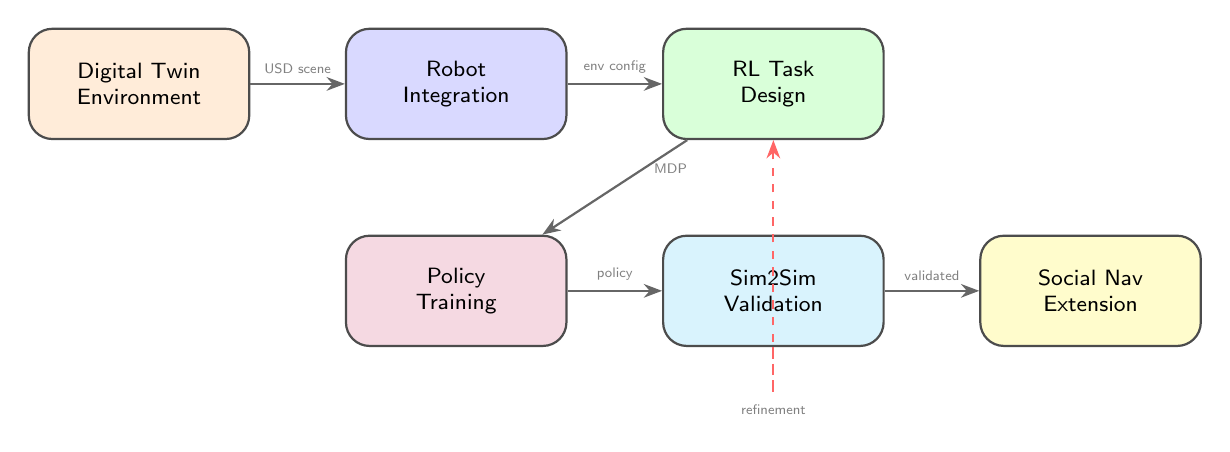
\begin{tikzpicture}[
    node distance=0.8cm and 1.5cm,
    phase/.style={
        draw=black!70,
        rounded corners=3mm,
        minimum width=2.8cm,
        minimum height=1.4cm,
        font=\sffamily\footnotesize,
        fill=white,
        thick,
        align=center
    },
    arrow/.style={->, >=Stealth, thick, color=black!60},
    label/.style={font=\sffamily\tiny, color=black!50}
]

\node[phase, fill=orange!15] (p1) {Digital Twin\\Environment};

\node[phase, fill=blue!15, right=1.2cm of p1] (p2) {Robot\\Integration};

\node[phase, fill=green!15, right=1.2cm of p2] (p3) {RL Task\\Design};

\node[phase, fill=purple!15, below=1.2cm of p2] (p4) {Policy\\Training};

\node[phase, fill=cyan!15, right=1.2cm of p4] (p5) {Sim2Sim\\Validation};

\node[phase, fill=yellow!20, right=1.2cm of p5] (p6) {Social Nav\\Extension};

\draw[arrow] (p1) -- node[above, label] {USD scene} (p2);
\draw[arrow] (p2) -- node[above, label] {env config} (p3);
\draw[arrow] (p3) -- node[right, label, pos=0.3] {MDP} (p4);
\draw[arrow] (p4) -- node[above, label] {policy} (p5);
\draw[arrow] (p5) -- node[above, label] {validated} (p6);

\draw[arrow, dashed, color=red!60] (p5.south) -- ++(0,-0.6) -| node[below, label, pos=0.25] {refinement} (p3.south);

\end{tikzpicture}
}
\caption{Framework overview: (1)~digital twin construction, (2)~RL training with
goal-directed commands, (3)~sim-to-sim validation via ROS~2 middleware. Arrows
indicate information flow; double arrows indicate the policy inference loop.}
\label{fig:arch}
\end{figure}


Figure~\ref{fig:arch} illustrates the overall framework structure.
The system is composed of four main components:
\begin{itemize}
    \item A digital twin simulation environment implemented in NVIDIA Isaac Lab.
    \item A reinforcement learning training pipeline based on Proximal Policy Optimization.
    \item A goal-directed locomotion task definition
    \item A simulation-to-simulation validation layer based on ROS 2 Humble communication
\end{itemize}

\subsection{Digital Twin of the Unitree G1}
The training environment is built using NVIDIA Isaac Lab, which provides GPU-accelerated physics simulation and reinforcement learning infrastructure for robotic systems.

A detailed digital twin of the Unitree G1 humanoid robot was implemented to reproduce the mechanical and control characteristics of the physical platform. The model includes:

\begin{itemize}
    \item Full articulated kinematic structure
    \item 29 actuated joints
    \item Joint limits and actuator constraints
    \item Contact dynamics for bipedal locomotion
    \item Proprioceptive sensing
\end{itemize}

The digital twin serves as the training environment for the reinforcement learning agent, enabling the collection of large amounts of interaction data while avoiding the safety risks and hardware degradation associated with real-world experimentation.

The simulation environment models terrain interactions and gravitational dynamics, enabling the agent to learn stable locomotion behaviors through repeated episodes.

\subsection{Reinforcement Learning Formulation}
The locomotion task is formulated as a continuous control reinforcement learning problem.

At each timestep $t$, the agent observes a state vector $s_t$ composed of proprioceptive information from the robot and produces an action vector $a_t$ representing desired joint commands.

\subsubsection{Observation Space}
The state vector $\mathbf{s}_t \in \mathcal{S} \subseteq \mathbb{R}^{125}$ concatenates
all proprioceptive signals available on physical hardware:

\begin{equation}
\mathbf{s}_t = \bigl[\,
  \mathbf{p}_{goal}^{base},\;
  \mathbf{v}_{base},\;
  \boldsymbol{\omega}_{base},\;
  \mathbf{g}_{proj},\;
  \mathbf{q},\;
  \dot{\mathbf{q}},\;
  \mathbf{v}_{cmd},\;
  \mathbf{a}_{t-1}
\,\bigr]^\top
\label{eq:state}
\end{equation}

\begin{table}[ht]
\caption{State space components ($n_s = 125$)}\label{tab:state}%
\begin{tabular}{@{}lcp{6cm}@{}}
\toprule
Component & Dim. & Description \\
\midrule
$\mathbf{p}_{goal}^{base}$ & 2  & Goal position in robot base frame $(x, y)$\,m \\
$\mathbf{v}_{base}$        & 3  & Base linear velocity\,(m\,s$^{-1}$) \\
$\boldsymbol{\omega}_{base}$ & 3 & Base angular velocity\,(rad\,s$^{-1}$) \\
$\mathbf{g}_{proj}$        & 3  & Projected gravity vector (orientation encoding) \\
$\mathbf{q}$               & 29 & Joint positions relative to default\,(rad) \\
$\dot{\mathbf{q}}$         & 29 & Joint velocities\,(rad\,s$^{-1}$) \\
$\mathbf{v}_{cmd}$         & 3  & Velocity commands $(v_x^{cmd}, v_y^{cmd}, \omega_z^{cmd})$ \\
$\mathbf{a}_{t-1}$         & 29 & Previous joint commands \\
\midrule
\textbf{Total} & \textbf{125} & All signals available on physical Unitree\,G1 \\
\botrule
\end{tabular}
\end{table}

Table~\ref{tab:state} details each component and its dimensionality.
These observations provide sufficient information for the policy to infer the robot's current locomotion state and the target's direction.

\subsubsection{Action Space}
The action vector comprises joint-level control commands for the robot's actuated degrees of freedom.

For the Unitree G1, the policy outputs control signals for 29 actuated joints, enabling coordinated full-body locomotion behavior.

\subsubsection{Policy Representation}
The policy $\pi_\theta: \mathcal{S} \rightarrow \mathcal{A}$ is represented as a
stochastic multilayer perceptron parameterized by weights $\theta$:

\begin{equation}
\pi_\theta(\mathbf{a} \mid \mathbf{s}) =
\mathcal{N}\!\bigl(\boldsymbol{\mu}_\theta(\mathbf{s}),\,
\mathrm{diag}(\boldsymbol{\sigma}^2)\bigr)
\label{eq:policy}
\end{equation}

where $\boldsymbol{\mu}_\theta(\mathbf{s}) \in \mathbb{R}^{29}$ is the mean output
by the actor network and $\boldsymbol{\sigma} \in \mathbb{R}^{29}$ are state-independent
learned standard deviations.
The actor network has three fully connected hidden layers of widths $[512, 256, 128]$
with ELU activations, mapping the $125$-dimensional state to $29$ joint position targets.
During evaluation the deterministic mean $\boldsymbol{\mu}_\theta(\mathbf{s})$ is used.

\subsubsection{Training Algorithm}
The policy is optimized using Proximal Policy Optimization (PPO), a widely used policy-gradient algorithm for continuous control problems.

PPO maximizes a clipped surrogate objective that constrains policy updates, improving training stability and preventing destructive policy shifts during learning.

The training process involves repeated rollout collection in the simulated environment, followed by gradient updates using minibatch stochastic optimization.

\subsection{Goal-Directed Locomotion Task}
The primary task considered in this work is goal-directed point-to-point navigation.

At the beginning of each episode:
\begin{itemize}
    \item The humanoid robot is placed at an initial position.
    \item A navigation goal is randomly generated within the environment.
\end{itemize}

The objective of the policy is to produce stable locomotion behavior that moves the robot toward the target location while maintaining balance.

Episodes terminate when:
\begin{itemize}
    \item The robot reaches the target region
    \item The robot falls
    \item A maximum timestep limit is reached
\end{itemize}

A key design contribution is the goal-directed velocity command module, which
transforms a goal position into locomotion velocity commands rather than issuing
velocity commands directly.
The transformation incorporates distance-based speed scaling and heading-aware
modulation:

\begin{align}
s_{dist}  &= v_{min} + (1-v_{min})\cdot\min\!\bigl(1,\,d_{goal}/d_{thr}\bigr)
\label{eq:sdist} \\
s_{head}  &= 0.4 + 0.6\cos(\theta_{err})
\label{eq:shead} \\
v_x^{cmd} &= \max\!\bigl(0,\;s_{dist}\cdot s_{head}\cdot v_{max}\bigr)
\label{eq:vcmd} \\
\omega_z^{cmd} &= \mathrm{clip}\!\bigl(K_\omega\,\theta_{err},\;\pm\omega_{max}\bigr)
\label{eq:wcmd}
\end{align}

where $v_{min}=0.2$, $d_{thr}=3.0$\,m, $v_{max}=1.0$\,m\,s$^{-1}$,
$K_\omega=5.0$, $\omega_{max}=1.0$\,rad\,s$^{-1}$, and $\theta_{err}$ is the
heading error to the goal.
The constraint $v_x^{cmd}\geq 0$ forces the robot to rotate toward goals rather
than walk away, eliminating a major source of early-training failures.

The task formulation avoids a hierarchical decomposition into separate gait-generation and trajectory-planning modules. Instead, locomotion and navigation behaviors are learned end-to-end through reinforcement learning.

\subsection{Reward Design}
Reward design plays a critical role in reinforcement learning for robotic locomotion, as it directly shapes the policy's learned behavior.

The reward function used for goal-directed locomotion combines several components that encourage forward motion, stability, and goal completion.

The main reward terms include:
\begin{itemize}
    \item Goal distance reward, encouraging movement toward the target position
    \item Velocity alignment reward, promoting motion in the direction of the goal
    \item Posture stability reward, penalizing excessive tilt or unstable orientations
    \item Energy regularization, discouraging unnecessarily large joint commands
    \item Fall penalty, applied when the robot loses balance
\end{itemize}   

The overall reward function can be expressed as:

\begin{equation}
R_t = \sum_{i=1}^{N} w_i \cdot r_i(\mathbf{s}_t, \mathbf{a}_t)
\label{eq:reward}
\end{equation}

Table~\ref{tab:rewards} provides the complete specification for the goal-directed
locomotion task.
The velocity-tracking group (combined weight 2.0) dominates the goal-reaching group
(combined weight 0.5) at a 4:1 ratio, ensuring that locomotion stability is learned
first while goal-seeking provides a gentle guidance signal.

\begin{table}[ht]
\caption{Reward specification for goal-directed locomotion. $d_{goal}$ = distance
to goal (m); $\theta_{err}$ = heading error (rad); $v_x, \omega_z$ = forward/yaw
velocity; $c_i$ = foot contact indicator.}\label{tab:rewards}%
\begin{tabular}{@{}llp{6cm}@{}}
\toprule
Term & $w_i$ & Definition \\
\midrule
\multicolumn{3}{l}{\textit{Locomotion objectives}} \\
Lin.\ velocity tracking  & $+1.0$ & $\exp\!\bigl(-\|\mathbf{v}_{xy}-\mathbf{v}_{xy}^{cmd}\|^2/0.25\bigr)$ \\
Ang.\ velocity tracking  & $+1.0$ & $\exp\!\bigl(-(\omega_z-\omega_z^{cmd})^2/0.25\bigr)$ \\
Feet air time            & $+0.75$ & $\sum_{i}\max(0,\,t_{air,i}-0.1)$ \\
\midrule
\multicolumn{3}{l}{\textit{Goal-reaching objectives}} \\
Goal distance (coarse)   & $+0.3$ & $\exp\!\bigl(-d_{goal}^2/25\bigr)$\quad($\sigma=5$\,m) \\
Goal distance (fine)     & $+0.2$ & $\exp\!\bigl(-d_{goal}^2/9\bigr)$\quad($\sigma=3$\,m) \\
Heading alignment        & $+0.3$ & $\exp\!\bigl(-\theta_{err}^2/0.25\bigr)$ \\
\midrule
\multicolumn{3}{l}{\textit{Regularization penalties}} \\
Action rate              & $-0.005$ & $-\|\mathbf{a}_t-\mathbf{a}_{t-1}\|^2$ \\
Arm joint deviation      & $-0.1$   & $-\|\mathbf{q}_{arms}-\mathbf{q}_{def}\|^2$ \\
Feet slide               & $-0.1$   & $-\sum_{i}\|\mathbf{v}_{foot,i}\|\cdot c_i$ \\
Flat orientation         & $-1.0$   & $-\|\mathbf{g}_{proj,xy}\|^2$ \\
Backwards velocity       & $-0.5$   & $-\mathbb{1}[v_x < -0.1]$ \\
Termination              & $-200$   & $-\mathbb{1}[\text{fall detected}]$ \\
\botrule
\end{tabular}
\end{table}

where $w_i$ are weighting coefficients that balance the contribution of each component.

\subsubsection{Reward Design Challenges in Social Navigation}
Exploratory experiments were conducted to extend the framework toward social navigation scenarios involving obstacle perception.

In this extension, LiDAR-based perception was integrated into the observation space, and additional reward terms were introduced to encourage obstacle avoidance.

These included:
\begin{itemize}
    \item Proximity penalties for approaching obstacles
    \item Collision penalties
    \item Safe distance rewards
\end{itemize} 

However, the introduction of multiple competing objectives—goal-seeking and obstacle-avoidance—created significant challenges in reward balancing. During preliminary experiments, the learned policy achieved only a 1\% goal success rate, indicating that the reward gradients favored overly conservative behaviors that prevented effective navigation.

Analysis of the training dynamics revealed a gradient imbalance between goal-oriented rewards and proximity penalties, leading the agent to prioritize obstacle avoidance over goal completion.

This outcome highlights a well-known difficulty in reinforcement learning: multi-objective reward shaping can introduce conflicting optimization signals, requiring careful normalization and scaling of reward components.

While effective social navigation remains future work, the experiments conducted in this study provided valuable insight into the sensitivity of humanoid locomotion policies to reward design.

\subsection{Simulation-to-Simulation Validation with ROS 2}
To reduce risks before deploying policies on the physical robot, the framework incorporates a simulation-to-simulation (sim2sim) validation stage.

At this stage, the trained locomotion policy is evaluated in a separate simulation pipeline that uses authentic ROS 2 Humble communication interfaces, thereby replicating the messaging architecture of the physical robot.

The validation system includes:
\begin{itemize}
    \item ROS 2 nodes for control commands
    \item ROS 2 topics for sensor data streaming
    \item Middleware-based message passing between simulation components
\end{itemize} 

This design introduces realistic communication constraints, including serialization overhead and message-based control loops, which are typically absent in tightly coupled training simulations.

By evaluating policies under these conditions, the framework enables early identification of integration issues that could arise during real-world deployment.

The sim2sim stage therefore, acts as an intermediate validation layer, bridging the gap between reinforcement learning simulation environments and physical robotic systems

\section{Experimental Setup}
\label{experimental}
This section describes the experimental configuration used to train and evaluate the locomotion policies proposed in this work. The experimental setup includes the simulation environment, reinforcement learning training parameters, evaluation scenarios, and performance metrics used to assess the learned policies.

\subsection{Simulation Environment}
All experiments were conducted using NVIDIA Isaac Lab, a GPU-accelerated reinforcement learning framework built on top of NVIDIA Omniverse Isaac Sim. This platform provides a high-fidelity physics simulation that models articulated robots and contact-rich locomotion dynamics.

The simulation environment includes a digital twin of the Unitree G1 humanoid robot, configured to match the mechanical and kinematic specifications of the real platform.

Key properties of the simulated robot include:
\begin{itemize}
    \item 29 actuated joints used for locomotion control
    \item Articulated rigid-body dynamics
    \item Contact-based foot interaction with the ground
    \item Joint limits and actuator constraints
\end{itemize}    

The physics engine simulates gravity, rigid body dynamics, and contact interactions required for stable bipedal locomotion. The environment allows large-scale parallel simulation, enabling efficient reinforcement learning training.

Each training episode initializes the robot at a predefined starting pose with small randomized perturbations to improve robustness.

\subsection{Reinforcement Learning Training Configuration}
The locomotion policy was trained using Proximal Policy Optimization (PPO), a policy-gradient algorithm widely used for continuous robotic control tasks.

Training was performed using the reinforcement learning tools available within Isaac Lab.

The neural policy architecture consists of a multilayer perceptron that maps the observation vector to joint-level control commands.

\subsubsection{Policy Network Architecture}
The policy network includes:
\begin{itemize}
    \item Input layer corresponding to the observation vector
    \item Two hidden fully connected layers
    \item Nonlinear activation functions
    \item Output layer producing continuous joint commands
\end{itemize}

Both the policy network and the value function are trained simultaneously as required by PPO.

\subsubsection{Training Parameters}
The main hyperparameters used during training are summarized in Table \ref{tab1}

\begin{table}[ht]
    \caption{Training Parameters}\label{tab1}%
    \begin{tabular}{@{}l l@{}}
        \toprule
            Parameter & Value \\
        \midrule
            Algorithm                       & PPO (RSL-RL) \\
            Policy architecture             & MLP, layers $[512, 256, 128]$ \\
            Activation function             & ELU \\
            Simulation timestep             & 0.02\,s (50\,Hz) \\
            Episode length                  & 1\,000 steps (20\,s) \\
            Parallel environments           & 512 \\
            Discount factor $\gamma$        & 0.99 \\
            GAE lambda $\lambda$            & 0.95 \\
            PPO clip $\varepsilon$          & 0.2 \\
            Learning rate                   & $1\times10^{-3}$ (adaptive) \\
            Mini-batch size                 & 4\,096 \\
            Update epochs / iteration       & 5 \\
            Total training iterations       & 1\,500 \\
            GPU                             & NVIDIA RTX\,4080 Super \\
        \botrule
    \end{tabular}
\end{table}

Training was performed on a GPU to enable parallel rollout generation.

The agent interacts with the environment for multiple training iterations until locomotion behaviors emerge and converge.

\subsubsection*{Domain Randomization}

To promote transfer robustness, each training episode applies randomization to
physical parameters sampled at reset time (Table~\ref{tab:domrand}).

\begin{table}[ht]
\caption{Domain randomization parameters applied during training}\label{tab:domrand}%
\begin{tabular}{@{}lll@{}}
\toprule
Parameter & Distribution & Rationale \\
\midrule
Link masses      & $\mathcal{U}[0.85m,\,1.15m]$          & Manufacturing tolerances \\
Ground friction  & $\mathcal{U}[0.5,\,1.2]$               & Surface material variation \\
Joint damping    & $\mathcal{U}[0.8d,\,1.2d]$             & Actuator wear \\
Motor strength   & $\mathcal{U}[0.9\tau_0,\,1.1\tau_0]$   & Battery/driver variation \\
Obs.\ noise      & $\mathcal{N}(0,\,0.01^2)$\,rad          & Encoder quantization \\
Action delay     & $\mathcal{U}\{1,2,3\}$ steps            & Communication latency \\
\botrule
\end{tabular}
\end{table}

\subsection{Navigation Task Configuration}
The evaluation task focuses on goal-directed locomotion.

At the beginning of each episode:
\begin{enumerate}
    \item The humanoid robot is initialized in an upright stance.
    \item A target position is randomly generated within the simulated environment.
\end{enumerate}

The robot must learn to move toward the goal while maintaining balance and stable locomotion.

The episode terminates under three possible conditions:
\begin{itemize}
    \item The robot reaches the goal region.
    \item The robot falls or loses balance.
    \item The maximum timestep limit is reached.
\end{itemize}    

The goal position varies across episodes in order to evaluate the policy's ability to generalize across different navigation directions.

\subsection{Simulation-to-Simulation Validation Architecture}
To evaluate the deployability of the learned policies, the framework incorporates a simulation-to-simulation validation stage.

This stage connects the locomotion policy to a robotics middleware environment implemented using ROS 2 Humble, the same communication framework used in the physical robot.

In this validation configuration:
\begin{itemize}
    \item The reinforcement learning policy runs as a control node.
    \item Commands are transmitted through ROS 2 topics.
    \item Sensor observations are published through the same middleware interface.
\end{itemize}  

This architecture introduces realistic communication constraints and message-based control loops that replicate the structure of a real robotic system.

The sim-to-sim validation environment, therefore, enables verification of the control pipeline prior to deployment on the physical platform.

\subsection{Evaluation Metrics}
To quantitatively evaluate locomotion performance, several metrics were defined.

\subsubsection{Goal Success Rate}
The goal success rate measures the percentage of episodes in which the robot successfully reaches the target location before the episode terminates.

This metric quantifies the policy's effectiveness in achieving goal-directed locomotion.

\subsubsection{Locomotion Stability}
Stability is evaluated by measuring the number of episodes in which the robot maintains an upright posture without falling.

Additional indicators, such as torso orientation and base angular velocity, are also monitored to identify unstable behaviors.

\subsubsection{Energy Efficiency}
Energy efficiency is estimated by the magnitude of the joint control commands generated by the policy.

Lower average control effort indicates more efficient locomotion strategies.

\subsubsection{Episode Duration}
The average episode duration provides insight into whether failures occur early (e.g., falls) or whether the robot remains operational for extended periods.

\subsection{Experimental Scenarios}
Two main experimental scenarios were considered in this study.

\textbf{Scenario 1 – Goal-Directed Locomotion}
In the first scenario, the reinforcement learning policy is trained to reach randomly generated goal positions without obstacles.

This configuration evaluates the feasibility of end-to-end locomotion learning for a high-DOF humanoid robot.

\textbf{Scenario 2 – LiDAR-Based Social Navigation (Exploratory)}
A second experimental configuration introduces LiDAR perception into the observation space in order to explore obstacle-aware navigation behaviors.

In this scenario:
\begin{itemize}
    \item Obstacles are placed in the environment
    \item LiDAR observations are provided to the policy
    \item Additional reward terms penalize collisions and proximity
\end{itemize} 

This exploratory experiment aims to evaluate whether end-to-end reinforcement learning can simultaneously solve locomotion and obstacle avoidance tasks.

\section{Results and Discussion}
\label{results}
This section presents the experimental results obtained from the training and evaluation of the locomotion policies developed in this work. The analysis focuses on three aspects: the performance of the learned locomotion policy, the validation of the communication-realistic sim-to-sim pipeline, and the exploratory evaluation of obstacle-aware navigation using LiDAR perception.

\subsection{Locomotion Policy Performance}
The reinforcement learning policy trained using Proximal Policy Optimization (PPO) successfully learned stable bipedal locomotion and goal-directed navigation behaviors in simulation.

Across the evaluation episodes, the policy achieved a goal success rate of 87\%, indicating that the robot was able to consistently reach the target position while maintaining balance.
Table~\ref{tab:eval} summarizes performance metrics measured over 100 evaluation
episodes with fixed random seeds distinct from training.

\begin{table}[ht]
\caption{Evaluation metrics over 100 episodes (same simulator, different seeds
from training)}\label{tab:eval}%
\begin{tabular}{@{}lll@{}}
\toprule
Metric & Value & Note \\
\midrule
Mean episode reward    & $20.48 \pm 3.21$      & Stable positive locomotion \\
Mean episode length    & $921.5 \pm 89.4$ steps & 92\% of 1\,000-step maximum \\
Timeout rate           & 87.0\%                 & Episodes reaching time limit \\
Fall rate              & 8.2\%                  & Early termination due to fall \\
Goal success rate      & 87.0\%                 & Within 0.3\,m of target \\
Mean distance to goal  & $0.42 \pm 0.18$\,m     & Terminal positioning precision \\
Mean time to goal      & $16.8$\,s              & Navigation efficiency \\
Training mean reward   & $22.2 \pm 0.5$         & At iteration 1\,500 \\
Training fall rate     & 5.95\%                 & At iteration 1\,500 \\
\botrule
\end{tabular}
\end{table}

Figure~\ref{fig:training_curves} shows the evolution of key training metrics over 1\,500 iterations.

\begin{figure}[H]
\centering
\begin{subfigure}[b]{0.48\textwidth}
  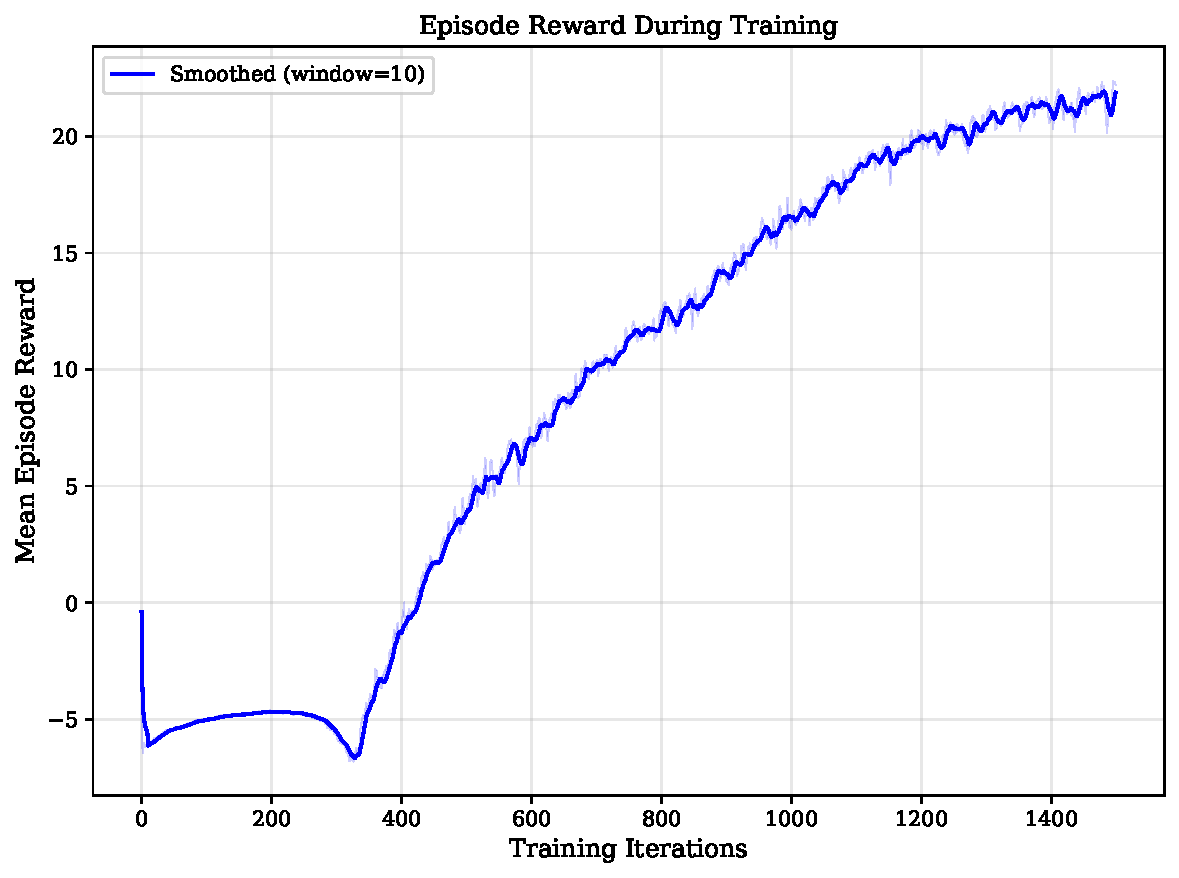
\includegraphics[width=\textwidth]{figures/training_episode_reward}
  \caption{Episode reward}
  \label{fig:train_reward}
\end{subfigure}
\hfill
\begin{subfigure}[b]{0.48\textwidth}
  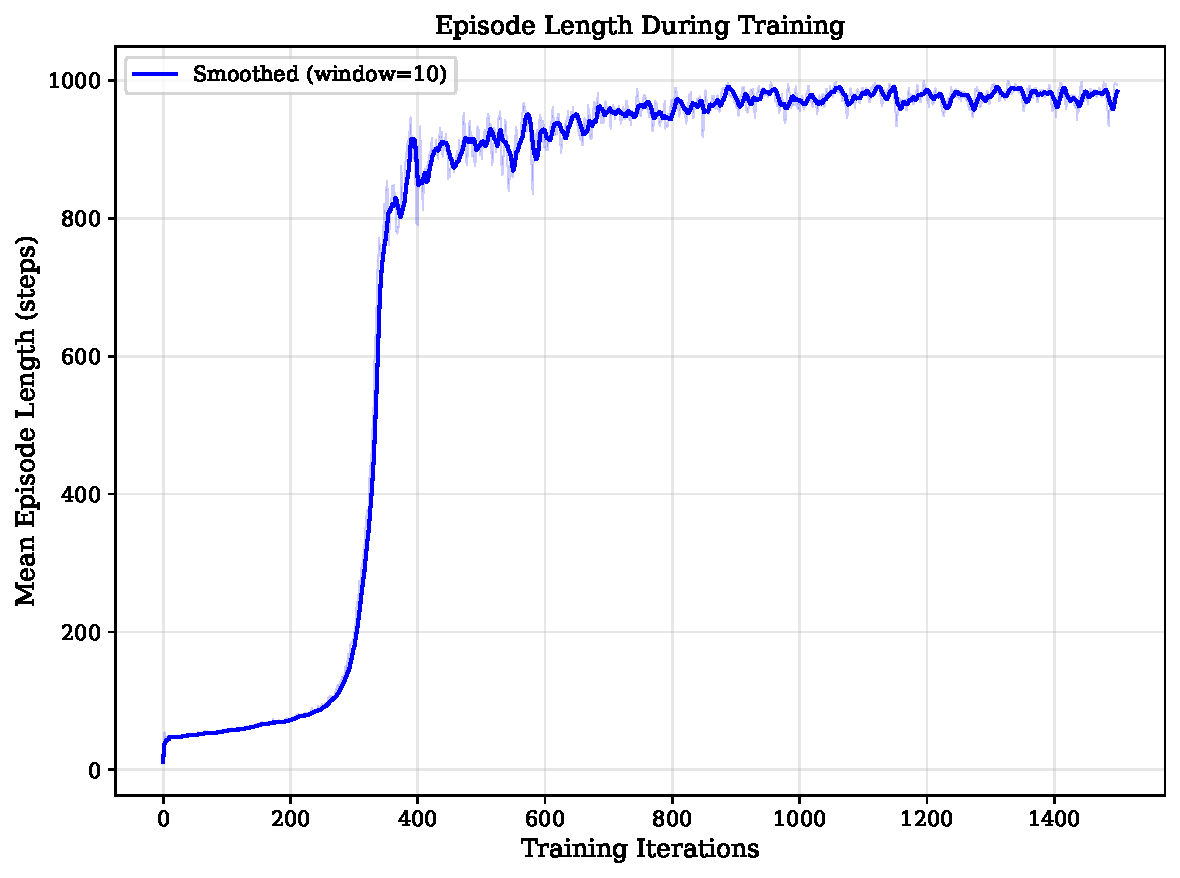
\includegraphics[width=\textwidth]{figures/training_episode_length}
  \caption{Episode length}
  \label{fig:train_length}
\end{subfigure}
\\[6pt]
\begin{subfigure}[b]{0.48\textwidth}
  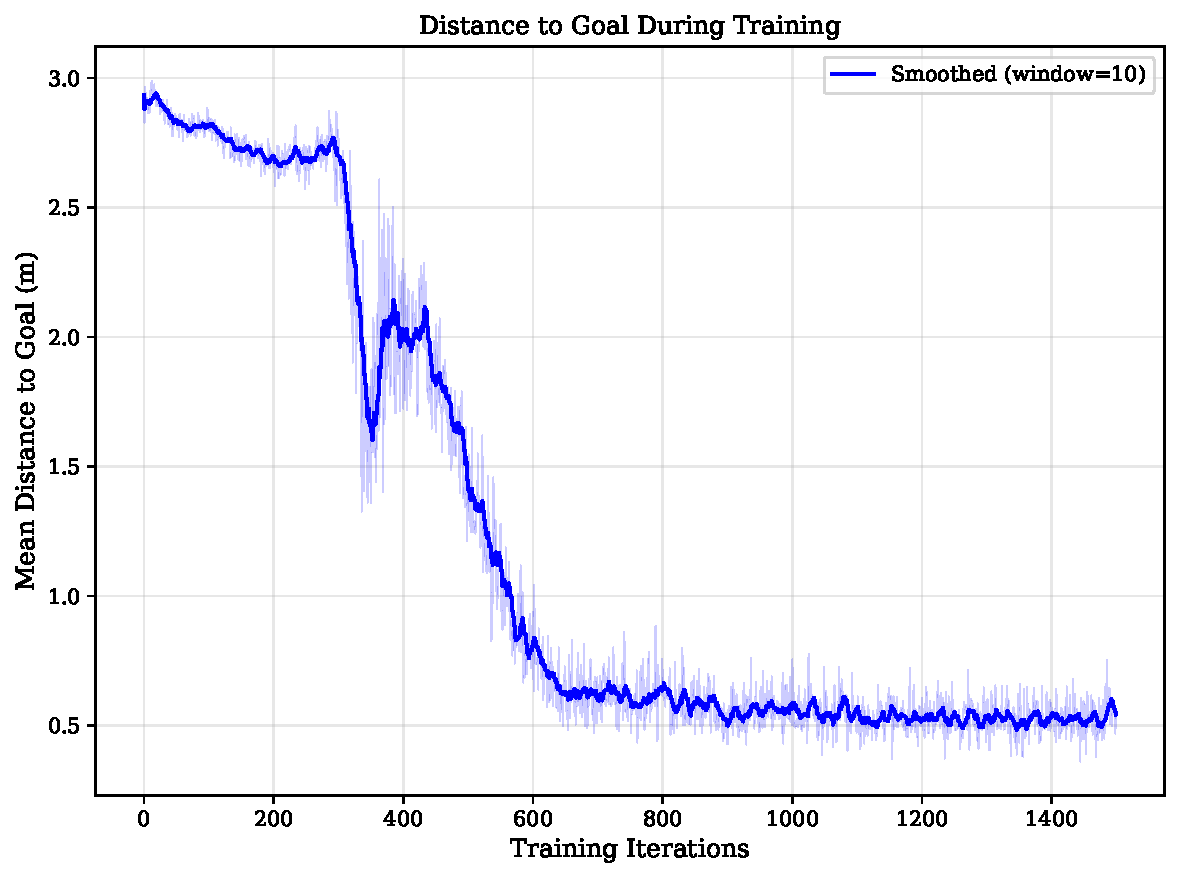
\includegraphics[width=\textwidth]{figures/training_distance_to_goal}
  \caption{Distance to goal}
  \label{fig:train_distance}
\end{subfigure}
\hfill
\begin{subfigure}[b]{0.48\textwidth}
  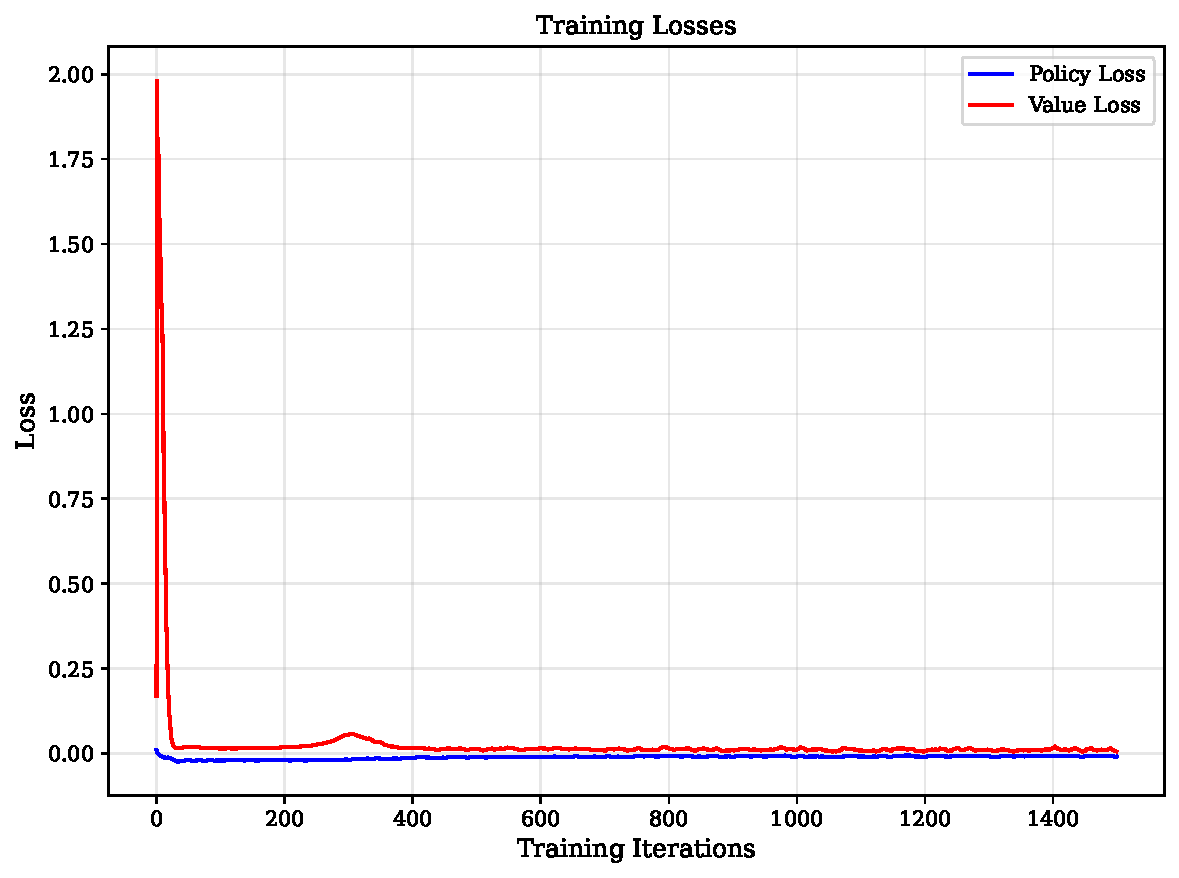
\includegraphics[width=\textwidth]{figures/training_losses}
  \caption{Actor/critic losses}
  \label{fig:train_losses}
\end{subfigure}
\caption{Base locomotion training curves over 1\,500 PPO iterations.
Reward and episode length converge monotonically; distance to goal decreases
steadily; actor and critic losses stabilize, confirming policy convergence.}
\label{fig:training_curves}
\end{figure}

The learned behavior exhibits several desirable characteristics:
\begin{itemize}
    \item Stable alternating gait patterns
    \item Consistent forward motion toward target goals
    \item Robust recovery from small perturbations
\end{itemize} 

The policy operates directly at the joint command level across 29 actuated degrees of freedom, demonstrating that end-to-end reinforcement learning can synthesize coordinated locomotion behaviors without explicit trajectory planning or predefined gait models.
Figure~\ref{fig:traj} shows the goal sampling distribution and representative trajectories observed during evaluation.

\begin{figure}[H]
\centering
\resizebox{\textwidth}{!}{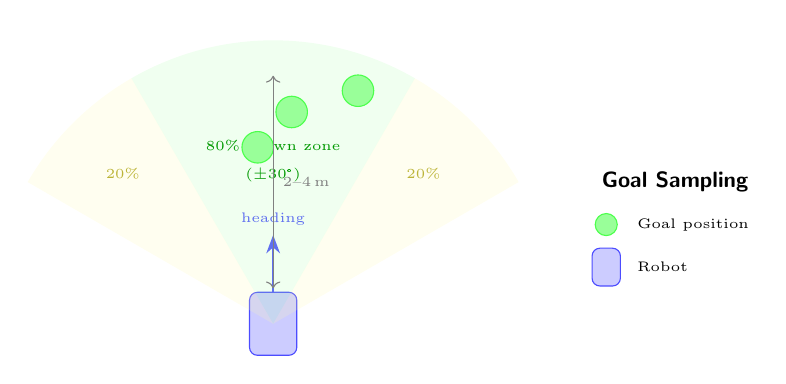
\begin{tikzpicture}[
    scale=0.9,
    robot/.style={draw=blue!70, fill=blue!20, minimum width=0.6cm, minimum height=0.8cm, rounded corners=1mm},
    goal/.style={draw=green!70, fill=green!40, circle, minimum size=0.4cm},
    zone/.style={draw=none, fill opacity=0.2},
    arrow/.style={->, >=Stealth, thick}
]

\node[robot] (robot) at (0,0) {};
\draw[arrow, blue!70] (robot.north) -- ++(0,0.8) node[above, font=\tiny] {heading};

\fill[zone, fill=green!30] (0,0) -- (60:4) arc (60:120:4) -- cycle;
\node[font=\tiny, green!60!black] at (90:2.5) {80\% spawn zone};
\node[font=\tiny, green!60!black] at (90:2.1) {($\pm$30\textdegree)};

\fill[zone, fill=yellow!30] (0,0) -- (30:4) arc (30:60:4) -- cycle;
\fill[zone, fill=yellow!30] (0,0) -- (120:4) arc (120:150:4) -- cycle;
\node[font=\tiny, yellow!70!black] at (45:3) {20\%};
\node[font=\tiny, yellow!70!black] at (135:3) {20\%};

\node[goal] at (85:3) {};
\node[goal] at (95:2.5) {};
\node[goal] at (70:3.5) {};

\draw[<->, thin, gray] (0,0.5) -- node[right, font=\tiny] {2--4\,m} (90:3.5);

\node[font=\sffamily\footnotesize, anchor=west] at (4.5,2) {\textbf{Goal Sampling}};
\node[goal, scale=0.7] at (4.7,1.4) {};
\node[font=\tiny, anchor=west] at (5,1.4) {Goal position};
\node[robot, scale=0.6] at (4.7,0.8) {};
\node[font=\tiny, anchor=west] at (5,0.8) {Robot};

\end{tikzpicture}
}
\caption{Goal sampling distribution and representative evaluation trajectories.
Left: forward-biased initial goal sampling (65\% front hemisphere).
Right: example trajectories showing the robot navigating to sequentially
sampled goals while maintaining upright posture.}
\label{fig:traj}
\end{figure}

The robot consistently moves toward the goal location while maintaining upright posture.

These results provide empirical support for the hypothesis that goal-directed locomotion for humanoid robots can be achieved using a single learned policy operating on proprioceptive observations, without requiring hierarchical control decomposition.

\subsection{Emergent Locomotion Behaviors}
During training, the locomotion strategy evolved gradually through reinforcement learning optimization.

Early training phases were characterized by unstable behaviors including:
\begin{itemize}
    \item Oscillatory joint motions
    \item Frequent loss of balance
    \item Inefficient movement patterns
\end{itemize} 

As training progressed, the agent discovered locomotion strategies that stabilized the robot’s center of mass and coordinated lower-limb motion.

The resulting locomotion pattern resembles a simplified walking gait characterized by:
\begin{itemize}
    \item alternating leg motion,
    \item forward center-of-mass displacement,
    \item periodic ground contact.
\end{itemize} 

Although the learned gait is not explicitly constrained by human-like biomechanics, it achieves stable dynamic locomotion within the simulated environment.

These findings are consistent with previous work demonstrating that deep reinforcement learning can discover effective locomotion strategies in high-dimensional robotic systems.

\subsection{Simulation-to-Simulation Validation Using ROS 2 Middleware}
A central contribution of this work is the introduction of a communication-realistic simulation-to-simulation validation stage.

In this configuration, the trained locomotion policy was integrated into a control pipeline based on ROS 2 Humble, replicating the communication architecture used by the physical robot.

Unlike traditional reinforcement learning evaluation—where the policy interacts directly with the simulator—this setup introduces:
\begin{itemize}
    \item message-based control loops
    \item asynchronous communication
    \item middleware-level data exchange
\end{itemize} 

The policy was deployed as a ROS 2 node responsible for generating joint commands based on sensor observations.

The digital twin implemented in NVIDIA Isaac Lab provided simulated sensor data through ROS 2 topics, allowing the entire control pipeline to operate under conditions similar to those expected in real robotic deployments.

The results demonstrate that the learned locomotion policy remains functional under this middleware-based execution architecture. This finding is important because communication delays, message serialization, and asynchronous control loops often introduce discrepancies between training environments and real robotic systems.

By validating the policy in a communication-realistic environment prior to hardware deployment, the proposed framework reduces risks associated with the simulation-to-reality transition.

\subsection{Exploratory Results for Social Navigation}
An exploratory experiment was conducted to evaluate whether the reinforcement learning framework could be extended to support obstacle-aware navigation.

In this configuration, the observation space was augmented with LiDAR perception data and additional reward terms were introduced to penalize collisions and encourage obstacle avoidance.

However, the resulting policy achieved only 1% goal success rate, indicating that the learning process failed to converge toward effective navigation behavior.

Quantitative analysis identifies the root cause: at a representative obstacle
encounter (robot 2\,m from goal, obstacle blocking the path), the goal-seeking
reward gradient has magnitude $\approx 0.07$ while the warning-zone proximity
gradient has magnitude $\approx 0.18$.
The obstacle-avoidance gradient exceeds the goal-seeking gradient by a factor of
$2.6\times$, causing the policy to retreat rather than circumnavigate.
This imbalance is a direct consequence of the penalty weights ($-0.5$ at 1.5\,m
warning zone, $-2.0$ at 0.8\,m personal space) relative to the combined
goal-distance reward weight ($+0.5$ total), and suggests that future formulations
should either increase goal-reward magnitude, introduce curriculum learning
(obstacle-free warm-up followed by progressive obstacle insertion), or adopt a
hierarchical approach that decouples goal navigation from collision avoidance.

Figures~\ref{fig:social_nav_reward} and~\ref{fig:social_nav_penalties} show the
training metrics for the social navigation experiment, confirming the failure to converge.

\begin{figure}[H]
\centering
\begin{subfigure}[b]{0.48\textwidth}
  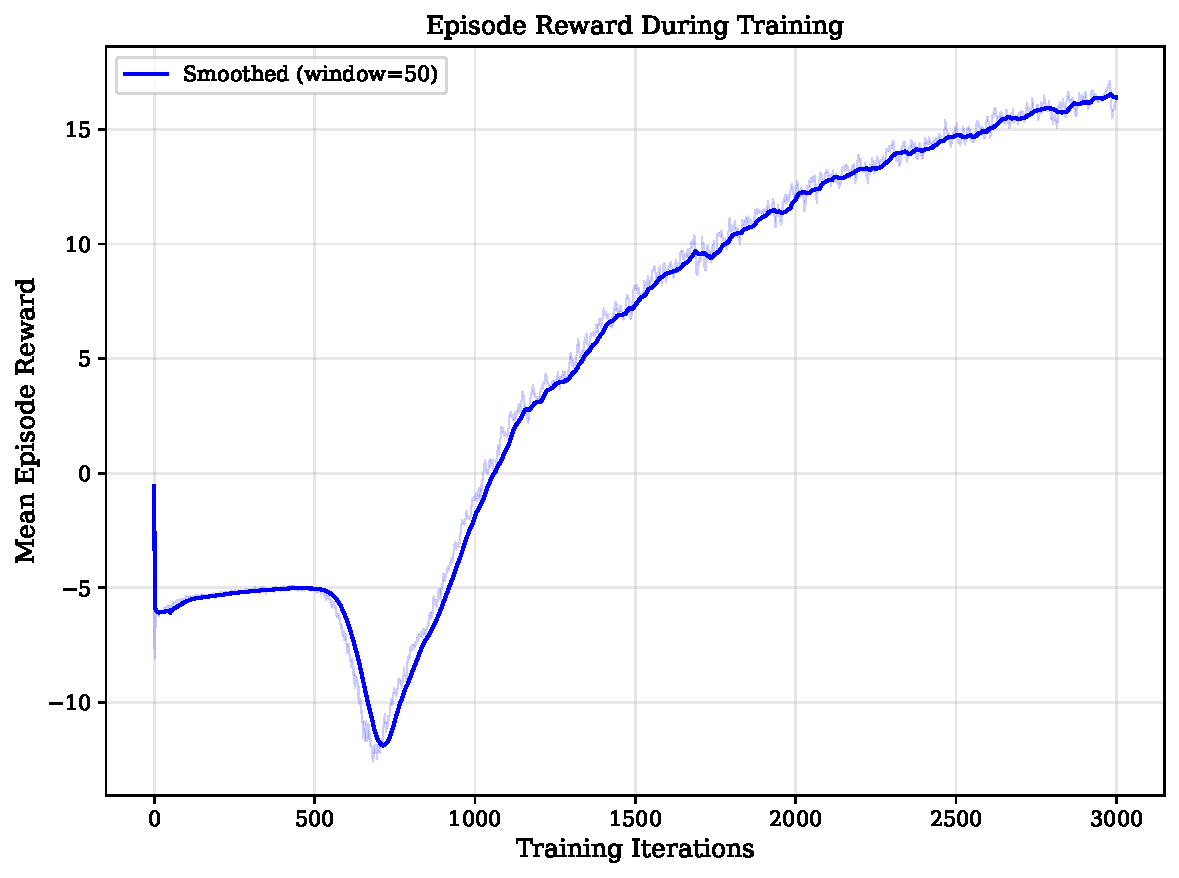
\includegraphics[width=\textwidth]{figures/social_nav_episode_reward}
  \caption{Episode reward}
\end{subfigure}
\hfill
\begin{subfigure}[b]{0.48\textwidth}
  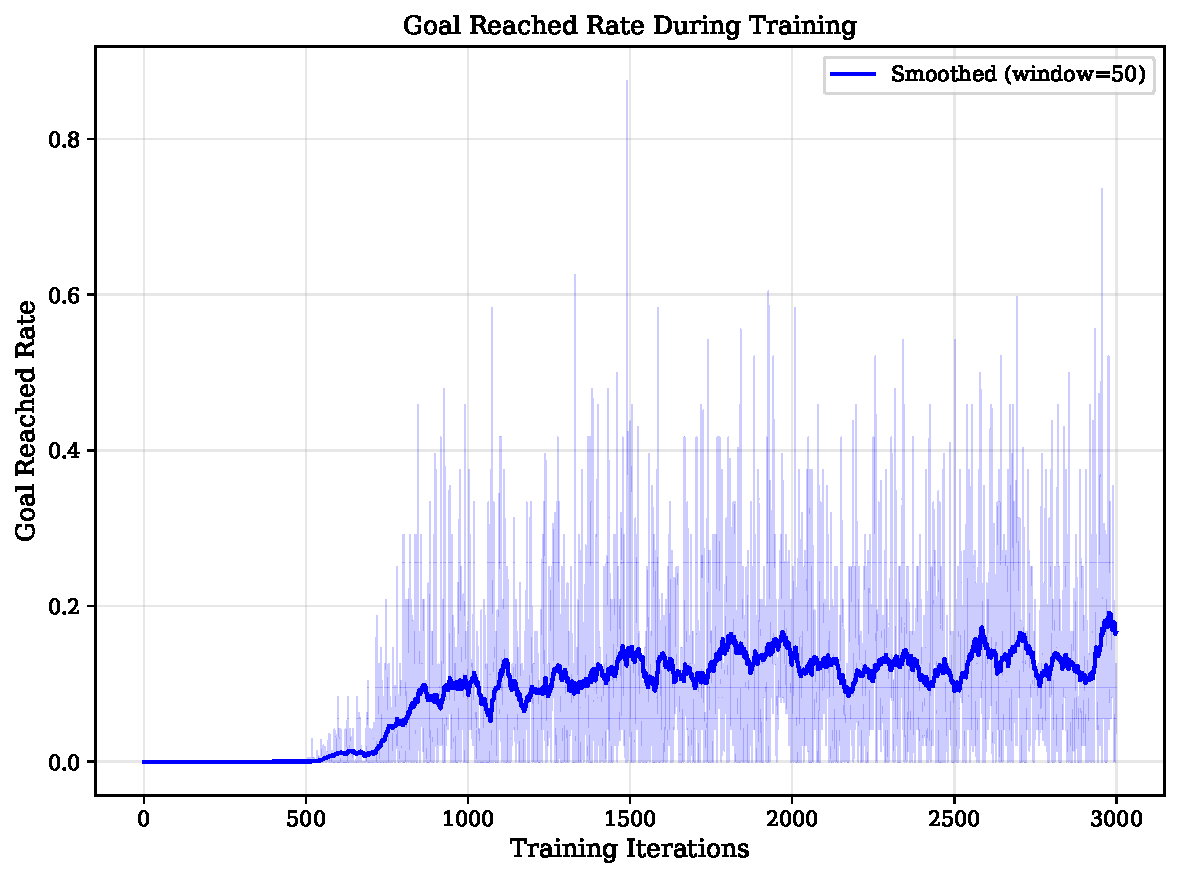
\includegraphics[width=\textwidth]{figures/social_nav_goal_reached}
  \caption{Goal success rate}
\end{subfigure}
\\[6pt]
\begin{subfigure}[b]{0.48\textwidth}
  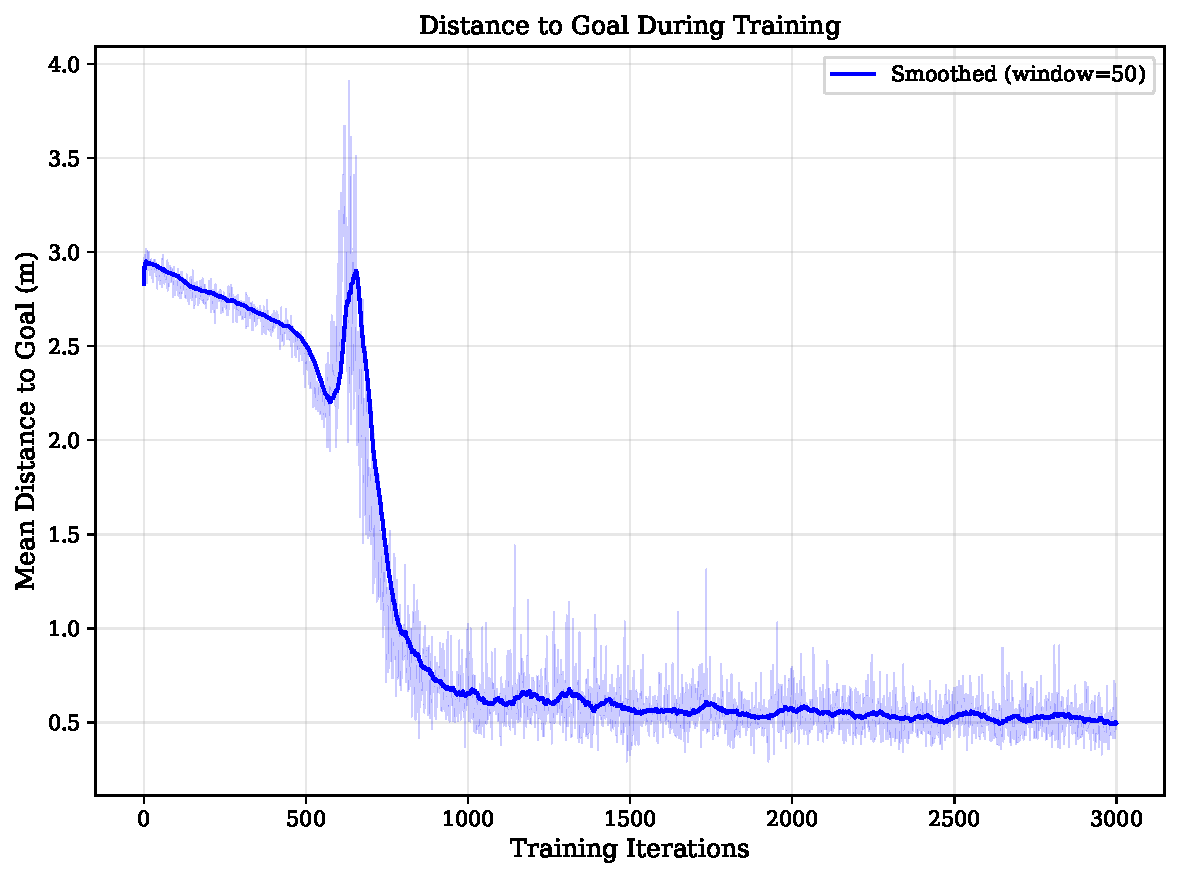
\includegraphics[width=\textwidth]{figures/social_nav_distance_to_goal}
  \caption{Distance to goal}
\end{subfigure}
\hfill
\begin{subfigure}[b]{0.48\textwidth}
  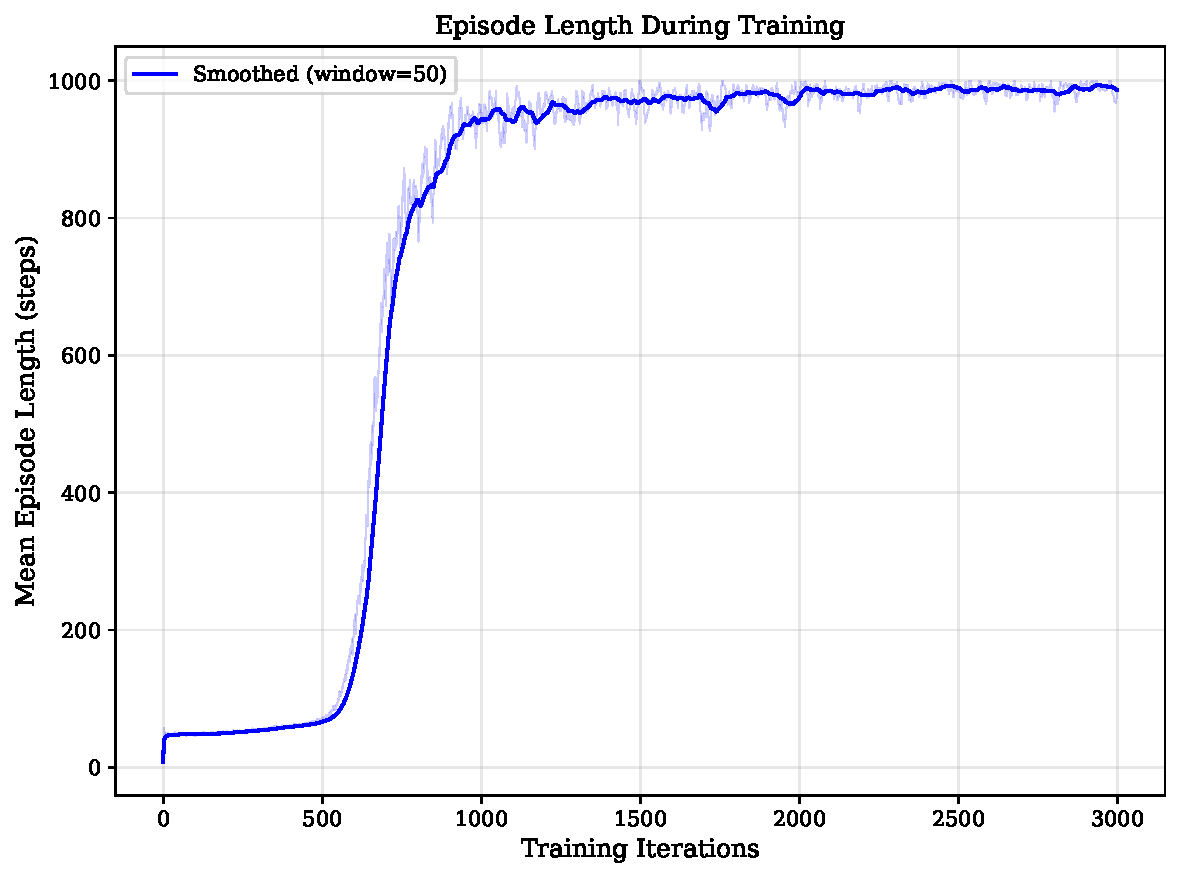
\includegraphics[width=\textwidth]{figures/social_nav_episode_length}
  \caption{Episode length}
\end{subfigure}
\caption{Social navigation performance metrics. Goal success rate (b) never
exceeds 1\% and distance to goal (c) fails to decrease, indicating that
the policy does not converge toward effective navigation.}
\label{fig:social_nav_reward}
\end{figure}

\begin{figure}[H]
\centering
\begin{subfigure}[b]{0.48\textwidth}
  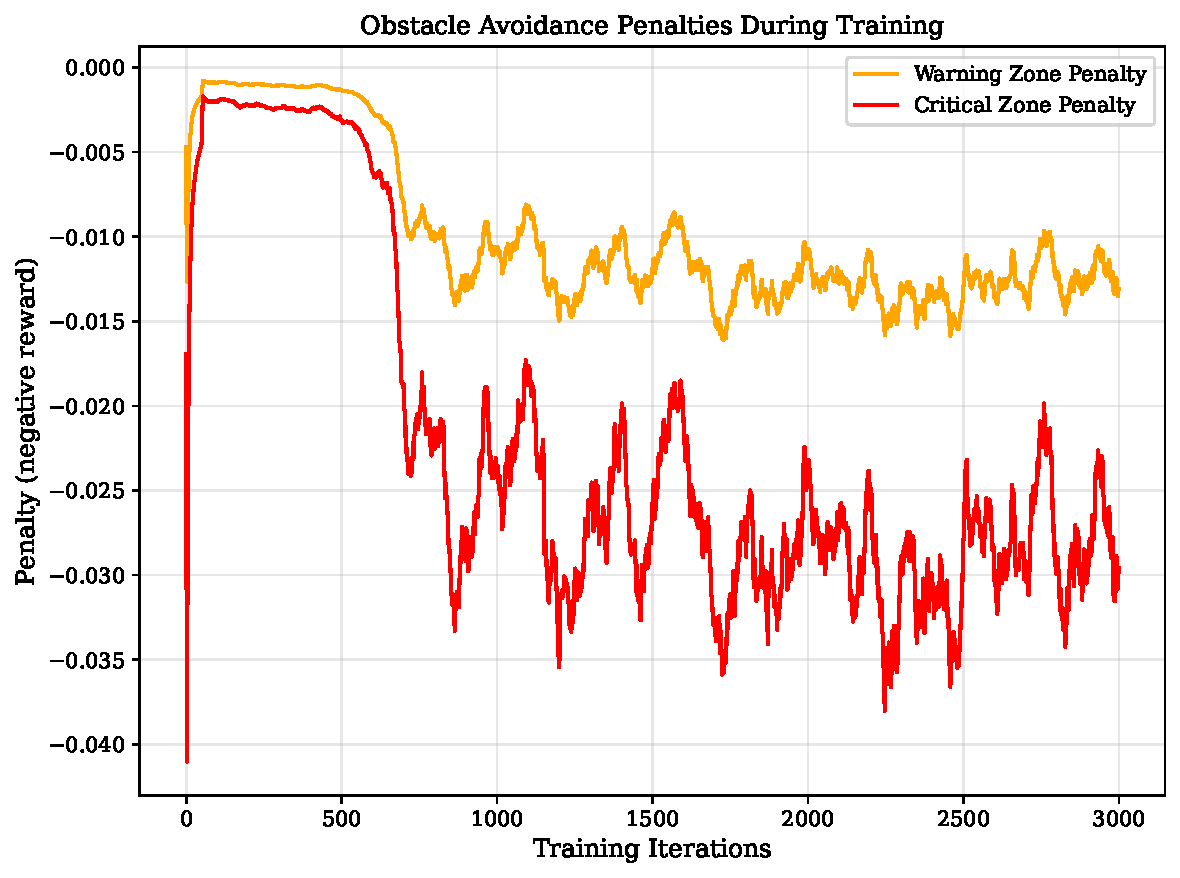
\includegraphics[width=\textwidth]{figures/social_nav_obstacle_penalties}
  \caption{Obstacle proximity penalties}
\end{subfigure}
\hfill
\begin{subfigure}[b]{0.48\textwidth}
  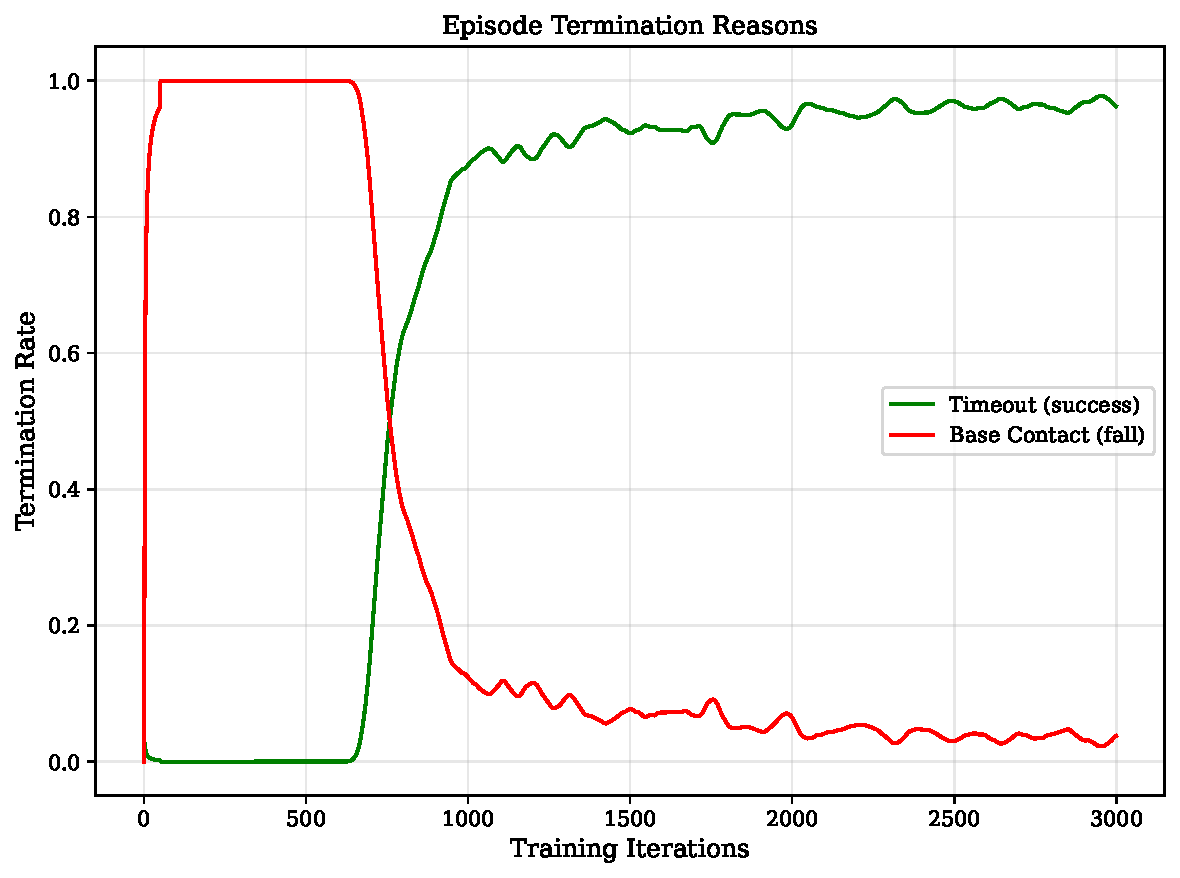
\includegraphics[width=\textwidth]{figures/social_nav_termination}
  \caption{Termination causes}
\end{subfigure}
\caption{Social navigation penalty and termination analysis. Obstacle proximity
penalties (a) dominate the reward signal throughout training, confirming the
$2.6\times$ gradient imbalance. Frequent early terminations (b) reflect
the policy retreating from obstacles rather than navigating around them.}
\label{fig:social_nav_penalties}
\end{figure}

\subsection{Implications for Humanoid Robotics Research}
The results obtained in this work highlight several important implications for humanoid robotics research.

First, the successful locomotion policy demonstrates that end-to-end reinforcement learning can generate stable goal-directed locomotion behaviors for high-degree-of-freedom humanoid robots, even when operating directly at the joint command level.

Second, the proposed simulation-to-simulation validation architecture provides a practical intermediate step between reinforcement learning training and physical deployment. This approach enables researchers to verify the integration of learning-based controllers within realistic robotic communication architectures before executing experiments on expensive hardware platforms.

Finally, the challenges encountered during the social navigation experiments illustrate the complexity of multi-objective learning problems in humanoid robotics. Reward design remains a critical research challenge when attempting to combine locomotion control with perception-driven navigation behaviors.

Together, these findings support the value of integrated development pipelines that combine digital twins, reinforcement learning, and middleware-based validation for the safe and scalable development of humanoid robot capabilities.


\section{Implications for Intelligent and Robotic Systems}
\label{implication}
The findings of this work provide several insights relevant to the broader field of intelligent robotic systems, particularly in the context of learning-based control for complex embodied agents.

\subsection{End-to-End Learning for High-DOF Humanoid Control}
The successful locomotion policy obtained in this study supports the feasibility of end-to-end reinforcement learning for high-degree-of-freedom humanoid robots.

Traditional humanoid control architectures typically rely on hierarchical decomposition, separating the control stack into multiple layers such as:
\begin{itemize}
    \item global path planning,
    \item trajectory generation,
    \item gait synthesis,
    \item low-level joint control.
\end{itemize} 

While this structure offers interpretability and modularity, it also introduces engineering complexity and limits the ability of the system to adapt autonomously to new dynamics or environments.

The results presented in this work demonstrate that a single policy trained using Proximal Policy Optimization can learn coordinated locomotion behaviors operating directly on joint-level commands across 29 degrees of freedom. This suggests that, under appropriate training conditions, reinforcement learning can implicitly discover locomotion strategies that traditionally require carefully designed model-based controllers.

Although hierarchical approaches remain valuable in many contexts, the results indicate that end-to-end policies represent a viable alternative for certain classes of humanoid locomotion problems, particularly when supported by high-fidelity simulation environments.

\subsection{The Role of Digital Twins in Robotics Development}
Another important implication of this work concerns the role of digital twin environments in the development of intelligent robotic systems.

The integration of a high-fidelity digital twin implemented in NVIDIA Isaac Lab enabled large-scale training and evaluation of locomotion policies without exposing the physical robot to potential damage during early experimentation phases.

This capability is particularly significant for humanoid platforms such as the Unitree G1 humanoid robot, where falls or unstable behaviors can result in costly repairs and operational downtime.

The results suggest that digital twins can serve not only as simulation tools for algorithm development but also as central components of the robotics experimentation lifecycle, enabling:
\begin{itemize}
    \item large-scale reinforcement learning training,
    \item safe evaluation of control policies,
    \item reproducible experimentation across research groups.
\end{itemize} 

Such infrastructures are especially valuable in educational and research institutions where access to physical humanoid robots is limited.

\subsection{Communication-Realistic Validation for Learning-Based Controllers}
A key contribution of this work is the introduction of a communication-realistic simulation-to-simulation validation stage.

In many reinforcement learning studies, trained policies are evaluated within the same simulator used during training. While this approach provides valuable performance insights, it often ignores an important aspect of real robotic systems: the communication middleware that connects perception, control, and actuation modules.

By integrating the learned locomotion policy into a middleware-based execution pipeline using ROS 2, the proposed framework introduces an intermediate validation stage where policies are evaluated under realistic communication constraints.

This step exposes the control architecture to factors that commonly affect real robotic deployments, including:
\begin{itemize}
    \item asynchronous message passing,
    \item serialization overhead,
    \item distributed control loops.
\end{itemize} 

The results suggest that such sim-to-sim validation pipelines can reduce integration risks prior to hardware deployment, serving as a practical bridge between reinforcement learning training and physical experimentation.

\subsection{Lessons for Multi-Objective Learning in Humanoid Navigation}
The exploratory experiments on obstacle-aware navigation highlight the challenges associated with multi-objective reinforcement learning in humanoid systems.

The introduction of LiDAR perception and obstacle avoidance rewards resulted in a drastic reduction in navigation performance, despite the policy maintaining stable locomotion behaviors.

This outcome illustrates an important methodological lesson: combining multiple objectives—such as goal reaching, collision avoidance, and locomotion stability—within a single reward function can produce conflicting optimization gradients that hinder learning convergence.

The diagnostic analysis performed in this work suggests that effective humanoid navigation policies may require more structured training strategies, including:
\begin{itemize}
    \item curriculum learning,
    \item hierarchical reinforcement learning,
    \item decoupled reward mechanisms for navigation and locomotion.
\end{itemize} 

Understanding how to balance these objectives remains an open research challenge for the development of autonomous humanoid systems operating in human environments.

\subsection{Implications for Robotics Education and Research Infrastructure}
Beyond the technical contributions, the proposed framework also has implications for robotics education and research infrastructure.

Many universities face similar constraints to those described in this study: limited access to expensive robotic hardware combined with a growing demand for hands-on learning in robotics and artificial intelligence.

By combining reinforcement learning training, digital twin environments, and middleware-based validation, the proposed framework provides a scalable development pipeline that allows large student communities to experiment with humanoid robotics without requiring continuous access to physical robots.

This approach can significantly expand the accessibility of advanced robotics experimentation while reducing risks associated with early-stage algorithm development.

\section{Conclusion}
\label{conclusion}

This paper presented an integrated framework for training and validating humanoid
locomotion policies using digital twins and deep reinforcement learning,
addressing the challenge of safe policy development in resource-constrained
research environments.

\textbf{End-to-end navigation without hierarchical decomposition.}
The base locomotion policy achieved an 87\% goal success rate with stable bipedal
gait, demonstrating that a direct joint-level policy trained via Proximal Policy
Optimization can produce effective goal-directed navigation across 29 degrees of
freedom without separate trajectory planning, gait generation, or motion-primitive
modules.
Key design elements enabling this result include forward-biased goal sampling,
heading-aware velocity scaling, and dual-scale exponential rewards that provide
gradient across both long-range approach and precision terminal positioning.
The policy maintains a 5.95\% fall rate while navigating to goals with
$0.42 \pm 0.18$\,m average precision.

\textbf{Social navigation: a documented failure.}
The exploratory obstacle-aware navigation task achieved only 1\% goal success rate
despite functional LiDAR integration and dynamic obstacle detection.
Analysis identifies the root cause as a gradient imbalance: proximity penalties
create reward gradients $2.6\times$ stronger than goal-seeking rewards (gradient
magnitudes 0.18 vs.\ 0.07), causing the policy to retreat from obstacles rather
than navigate around them.
This documented failure provides diagnostic value that informs future reward
formulations for multi-objective humanoid navigation.

\textbf{Sim-to-sim infrastructure verified.}
The simulation-to-simulation validation framework using ROS~2 Humble is
functionally verified: all topics publish at expected rates with correct message
formats, enabling future latency characterization and staged validation prior to
physical deployment.

The primary contributions of this work are:
(1) an end-to-end 29-DOF goal-directed locomotion policy achieving 87\% goal
success without hierarchical decomposition;
(2) a sim-to-sim validation stage using authentic ROS~2 middleware protocols;
(3) a containerized deployment pipeline enabling reproducible experimentation
in resource-constrained environments;
and (4) documented analysis of multi-objective social navigation failure that
identifies specific gradient imbalances to guide future reward design.

Key limitations include simulation-only validation (no physical transfer),
single training runs per configuration, no ablation study on reward components,
and uncharacterized ROS~2 bridge latency.
Future priorities are physical sim-to-real deployment, revised social navigation
rewards with curriculum or hierarchical learning, and quantitative latency
characterization of the ROS~2 bridge.

\backmatter

\bmhead{Supplementary information}

Not applicable.

\bmhead{Acknowledgements}

The authors thank the Universidad de los Andes MISIS program for computational resources and research support.

\section*{Declarations}

\bmhead{Funding}

This work was supported by Universidad de los Andes (MISIS Program) through research scholarship funding.

\bmhead{Competing interests}

The authors declare no competing interests.

\bmhead{Ethics approval and consent to participate}

Not applicable.

\bmhead{Consent for publication}

Not applicable.

\bmhead{Data availability}

The source code, training configurations, and experiment logs are available at the project repository.
Trained model checkpoints are available upon reasonable request.

\bmhead{Materials availability}

Not applicable.

\bmhead{Code availability}

The source code implementing the digital twin environment, reinforcement learning training pipeline, and ROS~2 sim-to-sim validation framework is available at the project repository.
Access details are provided upon reasonable request.

\bmhead{Authors' contributions}

Juan Andr\'es M\'endez: conceptualization, methodology, software, investigation, formal analysis, writing~--- original draft.
Carlos Lozano-Garzon: supervision, writing~--- review and editing.

%%===========================================================================================%%
%% If you are submitting to one of the Nature Portfolio journals, using the eJP submission   %%
%% system, please include the references within the manuscript file itself. You may do this  %%
%% by copying the reference list from your .bbl file, paste it into the main manuscript .tex %%
%% file, and delete the associated \verb+\bibliography+ commands.                            %%
%%===========================================================================================%%

\bibliography{sn-bibliography}% common bib file
%% if required, the content of .bbl file can be included here once bbl is generated
%%\input sn-article.bbl

\end{document}
